\chapter{身体活动与健康}\label{ch:g10:sport-and-health}

两名学生都十六岁。一人步行上学，每周打两次篮球，每晚睡八小时；
另一人被车接送，晚上坐在屏幕前，只睡六小时。
十六岁时，两人看起来相差无几。
到五十岁时，医生看到的将是两个不同的人：前者的心脏、骨骼、肌肉和血糖，
与年轻二十岁者相仿；后者则有一长串病症，
清单的开头是“慢性”一词。
前三章已说明工作中的身体如何运作；
本章讨论规律运动使它发生什么变化——
以及过度\omterm{def:g10:sport-and-health:training}{训练}或服药等滥用会破坏什么。

\section{训练带来的变化}

\begin{definition}[身体活动与训练]\label{def:g10:sport-and-health:training}
\emph{身体活动}\index{身体活动}是指由肌肉带动身体产生的、使\omterm{def:g10:exercise-and-energy:expenditure}{能量消耗}高于静息水平的任何运动，
如步行、爬楼梯、做家务和体育运动。\emph{训练}是
为提高某种能力而反复进行的身体活动。身体对反复出现的负荷
会以\emph{适应}作出反应：增大、增强或重新装备
所受负荷作用的结构——前提是
负荷之后有休息，
适应正是在休息中
形成。
\end{definition}

\begin{proposition}[耐力训练的适应]\label{prop:g10:sport-and-health:endurance}
时长较长、强度中等的反复运动，持续数月后，
会产生以下效果：
\begin{itemize}
  \item 心脏增大、增强：每搏输出量增加，静息
        心率下降（由 70 降至 50 或更低），最大输出量与
        $\dot V\!\mathrm{O_2}$max 提高 10\% 至 30\%；
  \item \omterm{def:g10:muscles-and-joints:muscle}{肌纤维}中的毛细血管和\omterm{def:g10:cells-common-unit:organelle}{线粒体}增多，
        它们能燃烧更多脂肪，
        在相同功率下产生的乳酸更少；
  \item 红\omterm{def:g10:cells-common-unit:cell}{细胞}增多，因而每升血液携带的氧气更多；
  \item \omterm{def:g10:exercise-and-energy:glycogen}{糖原}储备增大，身体更容易调节血糖
        与血压。
\end{itemize}
\end{proposition}
\admitted

\begin{omfigure}
\begin{tikzpicture}
\begin{axis}[
  width=0.86\linewidth, height=5.6cm,
  axis x line=bottom, axis y line=left,
  xmin=0, xmax=26, ymin=40, ymax=80,
  xlabel={训练周数}, ylabel={静息心率（次/分）},
  xlabel style={font=\small, at={(axis description cs:0.5,-0.12)}, anchor=north},
  ylabel style={font=\small},
  tick label style={font=\small}, xtick={0,4,8,12,16,20,24}, ytick={40,50,60,70,80},
  legend style={at={(0.5,-0.3)}, anchor=north, legend columns=2, font=\small, draw=none},
]
\addplot[thick, omThm, mark=*, mark size=1.5pt] coordinates
  {(0,72) (4,68) (8,64) (12,60) (16,57) (20,55) (24,54)};
\addplot[thick, omDef, mark=square*, mark size=1.5pt] coordinates
  {(0,72) (4,70) (8,66) (12,64) (16,62) (20,61) (24,61)};
\legend{每周 4 次, 每周 2 次}
\end{axis}
\end{tikzpicture}

{\small 两组初学者跑步六个月间的静息心率。心率下降
反映每搏输出量增大：静息时以更少的搏动输出同样的
\qty{5}{L/min}。适应程度与负荷成正比，
并随身体接近新的状态而放缓。}
\end{omfigure}

\begin{example}[适应的数据]\label{ex:g10:sport-and-health:numbers}
一名久坐的 17 岁青少年，$\dot V\!\mathrm{O_2}$max 为
每千克体重 \qty{40}{mL/min}，每周跑步三次，持续六个月后
升至 \num{48}，静息心率由 72 降至 58。他的肌肉
活检显示，每根纤维中\omterm{def:g10:cells-common-unit:organelle}{线粒体}多 40\%，毛细血管多 30\%。
他的\omterm{def:g10:muscles-and-joints:muscle}{肌纤维}数目与类型均未改变，
只是被重新装备了。
\end{example}

\begin{proposition}[力量训练的适应]\label{prop:g10:sport-and-health:strength}
反复对抗大负荷的收缩，使\omterm{def:g10:muscles-and-joints:muscle}{肌纤维}增粗（每根中的肌原纤维增多），
并改善募集它们的神经指令；
力量可在一年内翻倍，而\omterm{def:g10:muscles-and-joints:muscle}{肌纤维}数目不变。
承受\omterm{def:g10:sport-and-health:training}{训练}负荷的\omterm{def:g10:muscles-and-joints:muscle}{肌腱}和骨也会增粗，只是较慢。
骨尤其如此：骨的形成与维持随其所承受的负荷而定。
青春期的积极活动，决定了老年时将被消耗的骨量；
一条被石膏固定的肢体，
数周内便会流失骨质。
\end{proposition}
\admitted

\section{身体活动与健康}

\begin{proposition}[规律身体活动对健康的影响]\label{prop:g10:sport-and-health:health}
规律的\omterm{def:g10:sport-and-health:training}{身体活动}——青少年每天相当于一小时中等强度活动，
成年人为半小时——可
降低最常见慢性病的风险：心脏和动脉疾病、
2 型糖尿病、多种癌症、骨质疏松、抑郁。它通过
上述适应实现这一点：心脏和血管在较低压力下工作，
肌肉易于从血液中摄取葡萄糖，骨骼
保持骨量，体重维持在健康范围之内。作用
很大，堪比戒烟的效果，而且它
不必是体育运动，只需活动即可。
\end{proposition}
\begin{proof}[证据]
追踪数万人数十年的研究发现，
人口中活动量最高的五分之一人群，
在相同年龄下的死亡率约为活动量最低的五分之一人群的一半，
其中大部分差异可归因于心脏病；
这一关系在扣除饮食、吸烟和社会条件的影响后依然成立，
并且呈梯度变化——活动量每增加一级，风险便降低一级。
让久坐的人参加步行计划的试验显示，
数月之内血压和血糖便会下降。
\end{proof}

\begin{omfigure}
\begin{tikzpicture}
\begin{axis}[
  ybar, bar width=16pt,
  width=0.8\linewidth, height=5.4cm,
  axis x line=bottom, axis y line=left,
  ymin=0, ymax=1.2, ylabel={相对死亡风险},
  ylabel style={font=\small},
  symbolic x coords={least active, low, moderate, high, most active},
  xtick=data, xticklabels={最不活跃, 较低, 中等, 较高, 最活跃}, tick label style={font=\small},
  xlabel={按每周活动量划分的人口五分位组},
  xlabel style={font=\small, at={(axis description cs:0.5,-0.14)}, anchor=north},
  enlarge x limits=0.15, ytick={0,0.2,0.4,0.6,0.8,1.0},
  nodes near coords, nodes near coords style={font=\scriptsize},
  every node near coord/.append style={/pgf/number format/fixed, /pgf/number format/precision=2},
]
\addplot[fill=omThm!50, draw=omThm] coordinates
  {(least active,1.00) (low,0.80) (moderate,0.70) (high,0.62) (most active,0.55)};
\end{axis}
\end{tikzpicture}

{\small 在一个大型成年人群中，随访二十年的死亡风险，相对于
活动量最低的五分之一人群（综合多项研究取整）。每提高一级活动量，
风险都会降低；最大的降幅出现在第一步，
即由完全不活动到有一定活动。}
\end{omfigure}

\begin{example}[血糖与肌肉]\label{ex:g10:sport-and-health:sugar}
工作中的肌肉无需借助激素胰岛素，即可从血液中摄取葡萄糖，
经过\omterm{def:g10:sport-and-health:training}{训练}的肌肉在两次运动之间对胰岛素仍更为敏感。
饭后快走，可以降低随之出现的血糖峰值；
久坐的身体若要储存同样的糖分却不活动，
则每年需要更多胰岛素，这正是通向
2 型糖尿病的道路，其机制将于最后一学年学习。
\end{example}

\section{过量、过快、方法不当}

\begin{proposition}[过度训练与损伤]\label{prop:g10:sport-and-health:overtraining}
适应是在休息期间形成的。若负荷被反复施加，而恢复不足，
即\omterm{def:g10:sport-and-health:training}{训练}次数过多或强度过大，超出组织在两次\omterm{def:g10:sport-and-health:training}{训练}之间的修复能力，
则会产生与适应相反的结果：
持续疲劳、静息心率上升、运动表现下降，
睡眠紊乱、频繁感染，以及在修复最慢的组织（见\cref{ch:g10:muscles-and-joints}）中
出现\omterm{def:g10:muscles-and-joints:muscle}{肌腱}炎与应力性骨折。
青少年受伤最常见的原因并非运动项目本身，
而是负荷增加的速率。
\end{proposition}
\admitted

\begin{example}[百分之十法则]\label{ex:g10:sport-and-health:tenpercent}
每周跑量增幅不超过 10\% 的跑者，
通常很少受伤；两周内把跑量翻倍的人，则常常受伤。
骨骼与\omterm{def:g10:muscles-and-joints:muscle}{肌腱}的适应以月计，肌肉与心脏的适应以周计：
慢速组织决定了负荷可以提高的节奏。
\end{example}

\begin{proposition}[兴奋剂]\label{prop:g10:sport-and-health:doping}
\emph{兴奋剂}\index{兴奋剂}是指使用某些物质或方法，
通过干扰机体的调节机制来提高运动表现，以替代\omterm{def:g10:sport-and-health:training}{训练}本应建立的
适应。每一种手段都模拟某种适应，
同时付出绕过这种适应的代价：
\begin{itemize}
  \item 激素促红\omterm{def:g10:cells-common-unit:cell}{细胞}生成素（EPO）或回输自身储存的血液，
        可增加红\omterm{def:g10:cells-common-unit:cell}{细胞}数量——并
        使血液变稠，以致在心脏或脑的血管中
        形成血栓；
  \item 由睾酮衍生的合成\omterm{def:g10:cell-metabolism:metabolism}{代谢}类固醇，使\omterm{def:g10:muscles-and-joints:muscle}{肌纤维}
        增粗——同时扰乱机体自身的激素、肝脏、
        心脏以及情绪；
  \item \omterm{prop:g10:sport-and-health:doping}{兴奋剂}掩盖疲劳——同时去除了
        保护心脏免于过热和力竭的警示；
  \item 生长激素，以及掩盖其他手段的药物，
        使这份清单完整。
\end{itemize}
\omterm{prop:g10:sport-and-health:doping}{兴奋剂}在比赛中被禁止，因为它不公平；
它之所以危险，是因为上述每种物质都会凌驾于
一项有其存在理由的调节机制之上。
\end{proposition}
\admitted

\begin{example}[EPO 的数字]\label{ex:g10:sport-and-health:epo}
红\omterm{def:g10:cells-common-unit:cell}{细胞}约占正常血液体积的 45\%。
EPO 的滥用使运动员的比例升至 55\% 甚至更高，血液变得如此黏稠，
以至于因睡眠而减慢的心脏无法推动它：数名年轻的自行车手，
在检测手段出现之前的几年里，他们在睡眠中丧生。
高原\omterm{def:g10:sport-and-health:training}{训练}则可在数周内使该数值提高两到三个百分点，
且受机体自身的调控。
\end{example}

\section{日常规则}

\begin{method}[安全训练]\label{met:g10:sport-and-health:rules}
\begin{enumerate}
  \item \emph{循序渐进}：每周将负荷增加约十分之一，
        并让骨骼和\omterm{def:g10:muscles-and-joints:muscle}{肌腱}决定节奏。
  \item \emph{热身与放松}：各十分钟，理由见
        \cref{ch:g10:muscles-and-joints}。
  \item \emph{补充水分}：一小时的剧烈运动会流失一至两升
        汗液；应及时补充，并加入少量食盐，不必等到口渴——
        体重流失 2\% 即会降低运动表现。
  \item \emph{按运动需要进食}：长时间运动前和运动中补充\omterm{def:g10:chemistry-of-life:families}{糖类}，
        运动后补充\omterm{def:g10:chemistry-of-life:families}{蛋白质}以促进修复
        （见\cref{ch:g10:exercise-and-energy}）；任何补充剂都无法取代
        多样化的膳食。
  \item \emph{休息}：睡眠是适应形成的时段；静息心率
        上升则是休息不足最早的信号。
  \item \emph{留意疼痛}：\omterm{def:g10:muscles-and-joints:joint}{关节}或\omterm{def:g10:muscles-and-joints:muscle}{肌腱}的剧烈疼痛是一种
        信号，而非障碍。
\end{enumerate}
\end{method}

\begin{omfigure}
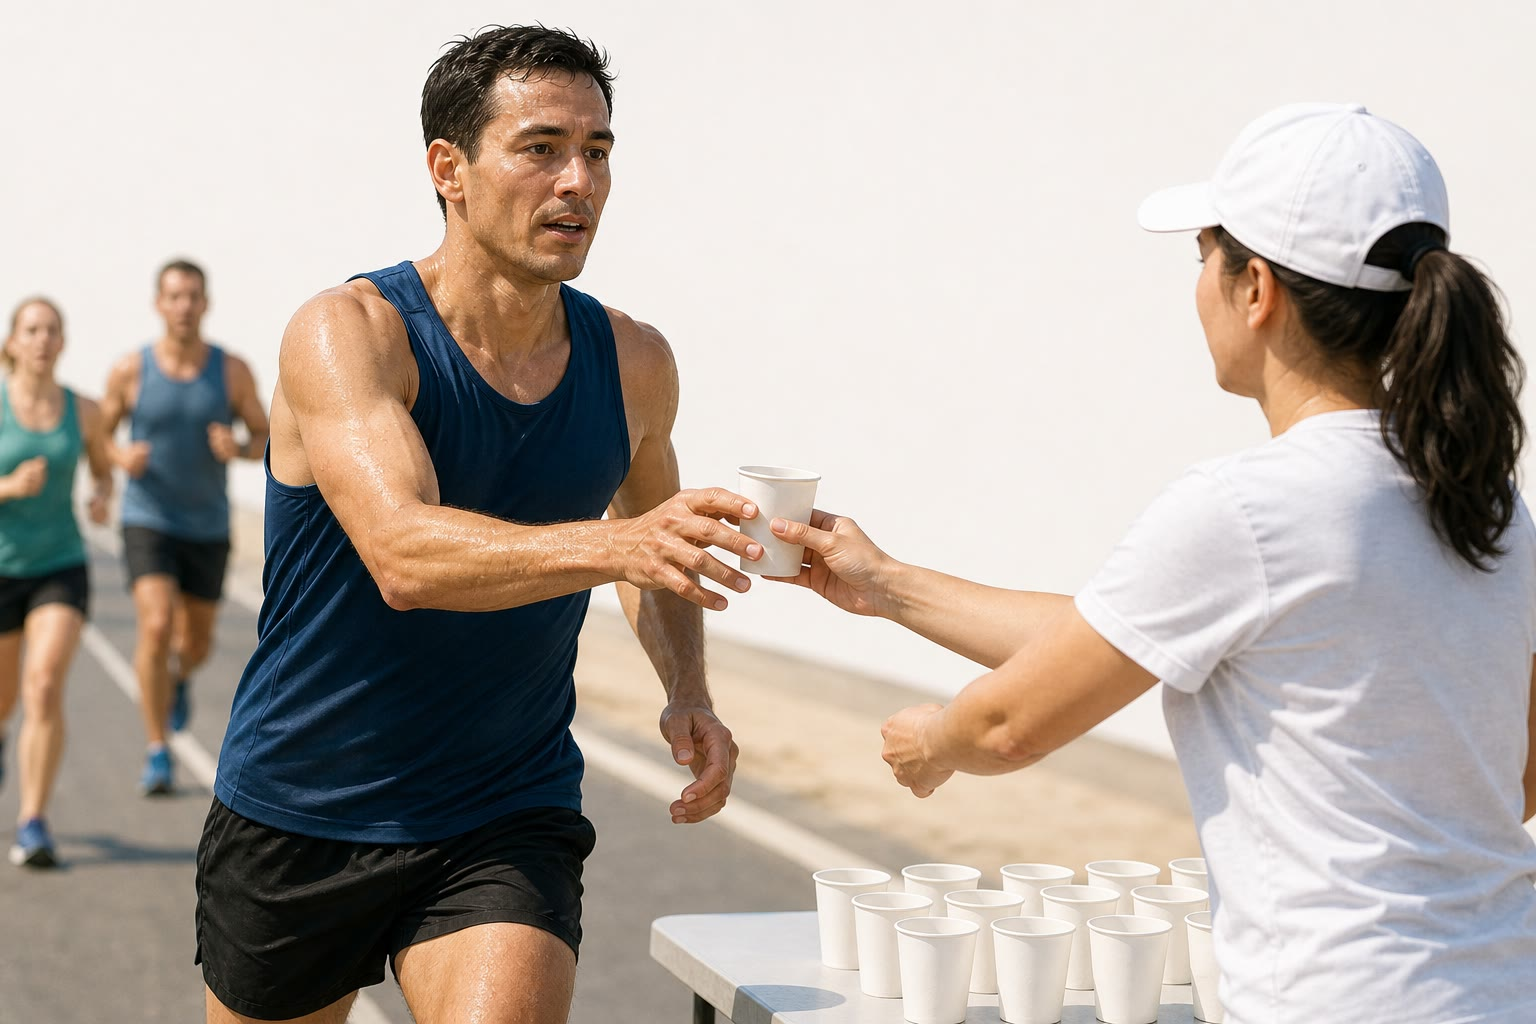
\includegraphics[width=0.62\linewidth]{images/book2/ai/g10-health-hydration.jpg}

{\small 马拉松赛道上的补给站。出汗速率
超过每小时一升时，运动中流失的水分必须及时补充；
等到口渴时再喝，就已经是脱水状态下跑步了。}
\end{omfigure}

\begin{example}[数字中的水合]\label{ex:g10:sport-and-health:water}
一名 \qty{60}{kg} 的跑者在温暖天气中每小时出汗 \qty{1.2}{L}。
跑两小时后她流失了 \qty{2.4}{kg}，占体重的 4\%：血容量下降，
为维持\omterm{def:g10:heart-lungs-effort:output}{心输出量}，心率上升了 10 次搏动，
体温升高，配速下降了十分之一。
每小时饮用半升水，本可使流失量减半。
\end{example}

\begin{remark}[身体记着这笔账]\label{rem:g10:sport-and-health:account}
本章中的每一种适应，都是身体为应对使用而构建的结构，
使用一旦停止，这些结构便会被逐一拆除：卧床一个月会使肌肉流失五分之一，
一年不活动则会丢失大部分耐力提升。
这笔账是持续计算的，
五十岁时的结余，
等于十六岁、二十六岁和三十六岁时存入之和。
\end{remark}

\section{练习}

\begin{exercise}[$\star$]\label{exo:g10:sport-and-health:1}
列出身体对耐力\omterm{def:g10:sport-and-health:training}{训练}的四种适应。
\end{exercise}

\begin{exercise}[$\star$]\label{exo:g10:sport-and-health:2}
为什么\omterm{def:g10:sport-and-health:training}{训练}后静息心率会下降，
而静息\omterm{def:g10:heart-lungs-effort:output}{心输出量}却不变？
\end{exercise}

\begin{exercise}[$\star$]\label{exo:g10:sport-and-health:3}
对青少年而言，每日推荐的\omterm{def:g10:sport-and-health:training}{身体活动}量是多少？
是否一定要是体育运动？
\end{exercise}

\begin{exercise}[$\star$]\label{exo:g10:sport-and-health:4}
给出\omterm{prop:g10:sport-and-health:doping}{兴奋剂}的定义，并举出两例，
说明各自违反了哪一项规定。
\end{exercise}

\begin{exercise}[$\star$]\label{exo:g10:sport-and-health:5}
说出过度\omterm{def:g10:sport-and-health:training}{训练}的三个征兆。
\end{exercise}

\begin{exercise}[$\star\star$]\label{exo:g10:sport-and-health:6}
根据心率图，比较两组在 12 周后心率
下降的幅度，并说明这反映了运动需求
与适应之间怎样的关系。
\end{exercise}

\begin{exercise}[$\star\star$]\label{exo:g10:sport-and-health:7}
某跑者静息时的输出量为 \qty{5.0}{L/min}。她的静息心率
在六个月内由 72 降至 54。她的每搏输出量
变为原来的多少倍？
\end{exercise}

\begin{exercise}[$\star\star$]\label{exo:g10:sport-and-health:8}
根据相对风险图，死亡风险在最活跃的五分之一人群中
比最不活跃者低了多少？哪一个单一措施
带来的收益最大？
\end{exercise}

\begin{exercise}[$\star\star$]\label{exo:g10:sport-and-health:9}
一名 \qty{55}{kg} 的学生在夏季进行两小时网球比赛，
每小时出汗 \qty{1.0}{L}，且未饮水。她流失了
占体重的多少比例？可能出现哪三种后果？
\end{exercise}

\begin{exercise}[$\star\star$]\label{exo:g10:sport-and-health:10}
一名初学者每周跑 \qty{10}{km}。按照每周增加百分之十的原则，
需要多少周才能达到每周 \qty{20}{km}？
（逐周计算，或注意 $1.1^7 \approx 1.95$。）
\end{exercise}

\begin{exercise}[$\star\star$]\label{exo:g10:sport-and-health:11}
解释为什么经过一年\omterm{def:g10:sport-and-health:training}{训练}，肌肉力量可以翻倍，
而\omterm{def:g10:muscles-and-joints:muscle}{肌纤维}的数量保持不变。
\end{exercise}

\begin{exercise}[$\star\star\star$]\label{exo:g10:sport-and-health:12}
某运动员血液中红\omterm{def:g10:cells-common-unit:cell}{细胞}占 45\%；滥用 EPO 后升至 56\%。利用
\cref{ch:g10:heart-lungs-effort}，估算每升血液携带的氧气增量，
进而估算 $\dot V\!\mathrm{O_2}$max 的增量，并解释这一增量
为何以致命血栓的风险为代价。
\end{exercise}

\begin{exercise}[$\star\star\star$]\label{exo:g10:sport-and-health:13}
在高海拔地区\omterm{def:g10:sport-and-health:training}{训练}三周，红\omterm{def:g10:cells-common-unit:cell}{细胞}从 45\% 升至 48\%；
在同样的时间内，EPO 使其升至 56\%。
尽管两者涉及的是同一种分子，
在什么意义上前者是一种适应，而后者不是？
\end{exercise}

\begin{exercise}[$\star\star\star$]\label{exo:g10:sport-and-health:14}
利用\cref{ex:g10:sport-and-health:sugar}，解释医生为何
给血糖开始升高的患者开出步行的处方，
以及这一处方为何比仅能降低血糖的药物
效果更好。
\end{exercise}

\begin{exercise}[$\star\star\star$]\label{exo:g10:sport-and-health:15}
“考试季之前的一个月高强度\omterm{def:g10:sport-and-health:training}{训练}，
能让我整年状态良好。”结合适应、休息，
以及不同组织的时间尺度，讨论这一说法。
\end{exercise}

\section{题目：两名学生，三十年}

\begin{problem}[{周末问题——一名积极活动与久坐的十六岁少年，
跟踪其训练、一段过度训练期，
以及他们的身体到中年时留下的账单}]
\label{pb:g10:sport-and-health:1}
亚历克斯和萨姆都十六岁，体重均为 \qty{62}{kg}，静息心率均为
72，$\dot V\!\mathrm{O_2}$max 为每千克 \qty{42}{mL/min}，
亚历克斯开始每周跑步三次，萨姆则不跑。

\medskip
\noindent\textbf{第一部分——亚历克斯\omterm{def:g10:sport-and-health:training}{训练}。}
六个月后，亚历克斯的静息心率降至 56，
每千克的 $\dot V\!\mathrm{O_2}$max 为 \qty{50}{mL/min}；其最大心率
（200）未变。
\begin{enumerate}
  \item 其静息\omterm{def:g10:heart-lungs-effort:output}{心输出量}仍为 \qty{4.8}{L/min}。计算
        \omterm{def:g10:sport-and-health:training}{训练}前后的每搏输出量。
  \item 分别计算\omterm{def:g10:sport-and-health:training}{训练}前后以升每分钟计的 $\dot V\!\mathrm{O_2}$max，
        并求增长的百分比。
  \item 假设其最大氧提取量（每升 \qty{150}{mL}）
        保持不变，计算\omterm{def:g10:sport-and-health:training}{训练}前后的最大\omterm{def:g10:heart-lungs-effort:output}{心输出量}，
        以及其最大每搏输出量，
        分别求\omterm{def:g10:sport-and-health:training}{训练}前后的值。
  \item 在
        \cref{prop:g10:sport-and-health:endurance}所述适应中，
        哪一种可解释每搏输出量的增加，
        哪一种可解释氧提取量的增加？
  \item 亚历克斯每周的跑步距离由 \qty{6}{km} 增至 \qty{24}{km}，
        六个月内完成。是否遵守了 10\% 规则？
        请写出计算过程。
\end{enumerate}

\medskip
\noindent\textbf{第二部分——亚历克斯过度\omterm{def:g10:sport-and-health:training}{训练}。}
春季，亚历克斯为准备比赛，两周内将跑步距离翻倍，
三周后：静息心率升至 64，睡眠质量差，感冒，
胫部疼痛，比赛用时变慢。
\begin{enumerate}[resume]
  \item 指出该状况的名称，并列出本章中与之相符的
        体征。
  \item 用
        \cref{ch:g10:muscles-and-joints}的术语，胫部疼痛最可能的原因是什么，
        以及为何是该组织？
  \item \omterm{def:g10:sport-and-health:training}{训练}曾经降低了静息心率，
        为何静息心率又会升高？
  \item 拟定一份为期三周的计划，并用
        \cref{met:g10:sport-and-health:rules}为计划的每一项提供依据。
  \item 一位队友推荐一种能消除疲劳的“补剂”，它属于
        \cref{prop:g10:sport-and-health:doping}中的哪一类，
        以及它违背了哪项规定？
\end{enumerate}

\medskip
\noindent\textbf{第三部分——萨姆久坐。}
三十岁时，萨姆体重 \qty{80}{kg}，静息心率为 78，
$\dot V\!\mathrm{O_2}$max 为每千克 \qty{32}{mL/min}；亚历克斯仍然
活跃，体重 \qty{64}{kg}，静息心率 54，另一项指标为 \num{48}。
\begin{enumerate}[resume]
  \item 计算两人以升每分钟计的 $\dot V\!\mathrm{O_2}$max；
        哪一个绝对值更大？
        为何日常生活中真正重要的是每千克的数值？
  \item 爬四段楼梯时，每人高于静息水平的耗氧量约为每千克体重每分钟
        \qty{12}{mL} 氧气。各自占其最大值的几分之几？
        谁会上气不接下气地
        到达？
  \item 萨姆的医生发现其血糖略高于正常值。
        结合\cref{ex:g10:sport-and-health:sugar}，解释其
        缺乏运动与血糖之间的联系。
  \item 医生开出每天快走半小时的处方。
        利用相对风险数据，估算
        萨姆从活动量最少的五分之一人群，
        转至中等活动量人群后，长期风险的降低幅度。
  \item 萨姆说他没有时间运动。请用
        \cref{def:g10:sport-and-health:training}回答他。
\end{enumerate}

\medskip
\noindent\textbf{第四部分——五十岁时的账单。}
\begin{enumerate}[resume]
  \item 骨量约在二十五岁时达到峰值，此后每年约下降
        1\%。若亚历克斯的峰值比萨姆高 10\%，
        是因为其青少年时期活跃，则这一差距相当于
        多少年的下降量？
  \item 萨姆五十岁时跌倒，腕部骨折，而亚历克斯
        没有骨折。请将此与第 16 题以及
        \cref{prop:g10:sport-and-health:strength}联系起来。
  \item 亚历克斯四十岁时因受伤中断\omterm{def:g10:sport-and-health:training}{训练}一年，
        大部分耐力提升随之丧失，之后又重新获得。这说明
        适应的本质是什么？
  \item 对五十岁时的萨姆，列出其缺乏运动使之更可能出现的三种
        \cref{prop:g10:sport-and-health:health}所述状况，
        并说明其中一种的发生机制。
  \item 陈述结论：使两人在三十岁时出现差异的两个数值（静息心率，
        每千克 $\dot V\!\mathrm{O_2}$max），以及
        每周以小时计的那一项习惯，
        正是它造成了这一差异。
\end{enumerate}
\end{problem}
